% !TeX root = ../libro.tex
% !TeX encoding = utf8

\chapter{Resultados}
En este capítulo se expondrá un análisis de los resultados obtenidos por los distintos modelos y se comentará su rendimiento en las bases de datos a las que se han aplicado.

\section{K Nearest Neighbours}
Se alcanza una precisión de 0.591 y de hasta un 0.6641 usando validación cruzada (\textit{cross validation} en inglés) con 5 particiones del conjunto. De media, la validación cruzada ha conseguido una precisión del 0.62347.\\
También se ha dibujado \cite{Hunter:2007} la matriz de confución para cada clasificador. La matriz representa el número de falsos y verdaderos positivos así como el de falsos y verdaderos negativos, se ha realizado con la librería \textit{scikit-learn} \cite{scikit2021metrics}, contando en forma de tabla las etiquetas que el modelo ha predicho y su verdadera etiqueta.

\begin{figure}[H]
\centering
\begin{minipage}[t]{.5\textwidth}
  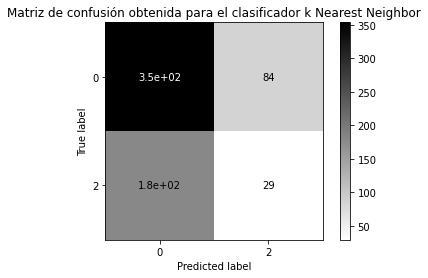
\includegraphics[width=\linewidth]{matriz_confusion_knn_trios}
  \caption{Matriz para KNN en tríos}
  \label{fig:confusion-knn-trios}
\end{minipage}%
\begin{minipage}[t]{.5\textwidth}
  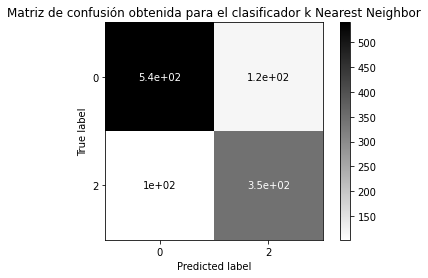
\includegraphics[width=\linewidth]{matriz_confusion_knn_control1}
  \caption{Matriz para KNN en el primer control}
  \label{fig:confusion-knn-control1}
\end{minipage}
\end{figure}

También con la librería \textit{metrics} de \textit{scikit-learn} se ha obtenido el valor para cada métrica:

\begin{table}[htpb]
  \centering
  \begin{tabular}{ccccc} \toprule
    \multicolumn{5}{c}{Conjunto de datos} \\ \cmidrule(r){1-5}
     & precision & recall & f1-score & support          \\ \midrule
    0 & 0.66 & 0.81 & 0.73 & 438          \\ 
    2 & 0.26 & 0.14 & 0.18 & 210          \\ 
    accuracy &  &  & 0.59 & 648          \\
    macro avg & 0.46 & 0.47 & 0.45 & 648          \\
    weighted avg & 0.53 & 0.59 & 0.55 & 648          \\ \bottomrule
  \end{tabular}
  \caption{Métricas obtenidas para K-NN en tríos}
  \label{tb:metricas-knn-trios}
\end{table}
Los resultados para este modelo, como se podía intuir en la representación gráfica de los SNPs, no es muy buena con un recall de 0.47 y una medida F1 de 0.18 para la etiqueda de afectado, el modelo predice bien a los no afectados debido al desbalance de los datos, es más probable que tenga cerca a más no afectados que a afectados, por ello, sólo ha predicho bien los individuos sanos.\\\\
Para los primeros datos de control se ha repetido el entrenamiento del mismo modelo dando una precisión de hasta 0.8136 en \textit{cross validation}. La tabla de métricas ha sido la siguiente:

\begin{table}[htpb]
  \centering
  \begin{tabular}{ccccc} \toprule
    \multicolumn{5}{c}{Conjunto de datos} \\ \cmidrule(r){1-5}
     & precision & recall & f1-score & support          \\ \midrule
    0 & 0.84 & 0.82 & 0.83 & 659          \\ 
    2 & 0.74 & 0.77 & 0.76 & 448          \\ 
    accuracy &  &  & 0.80 & 1107          \\
    macro avg & 0.79 & 0.80 & 0.79 & 1107          \\
    weighted avg & 0.80 & 0.80 & 0.80 & 1107          \\ \bottomrule
  \end{tabular}
  \caption{Métricas obtenidas para K-NN en el primer control}
  \label{tb:info-datasets}
\end{table}
Esta vez los datos estaban más balanceados y a simple vista más diferenciados entre padres de afectados y individuos sanos, con lo que se han logrado mejores resultados.

\section{Regresión Logística}
Los coeficientes de cada variable en la regresión logística indican el grado de importancia en el entrenamiento del modelo, así que se han ordenado los SNPs según su importancia quedando de la siguiente forma los diez más importantes:

\begin{figure}[H]
  \centering
  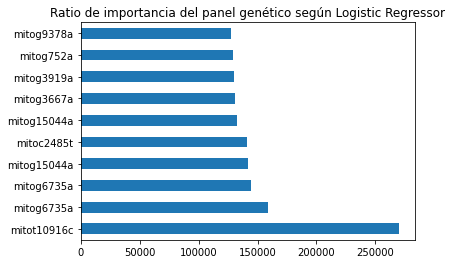
\includegraphics[width=0.45\textwidth]{importancia_rl_trios}
  \caption{Ratio de importancia Regreción Logística en tríos}
  \label{fig:k-nn-example}
\end{figure}

La importancia en estos diez primeros es muy parecida entre sí, con valores de coeficientes relativamente bajos, loo que lleva a pensar que para el modelo no ha habido ningún alelo especialmente significativo.\\
Se muestra a continuación la matriz de confusión y las métricas obtenidas para el modelo:

\begin{figure}[H]
\centering
\begin{minipage}[t]{.5\textwidth}
  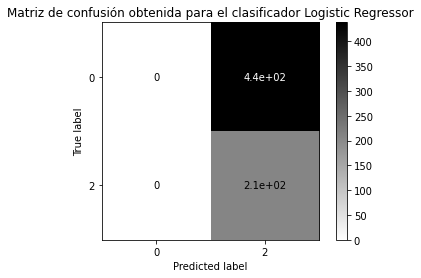
\includegraphics[width=\textwidth]{matriz_confusion_rl_trios}
  \caption{Matriz para RL en tríos}
  \label{fig:k-nn-example}
\end{minipage}%
\hfill
\begin{minipage}[t]{.5\textwidth}
  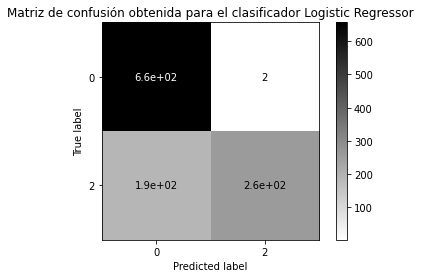
\includegraphics[width=\linewidth]{matriz_confusion_rl_control1}
  \caption{Matriz para RL en el primer control}
  \label{fig:confusion-knn-control1}
\end{minipage}
\end{figure}

\begin{table}[H]
  \centering
  \begin{tabular}{ccccc} \toprule
    \multicolumn{5}{c}{Conjunto de datos} \\ \cmidrule(r){1-5}
     & precision & recall & f1-score & support          \\ \midrule
    0 & 0.66 & 0.51 & 0.58 & 438          \\ 
    2 & 0.31 & 0.46 & 0.37 & 210          \\ 
    accuracy &  &  & 0.49 & 648          \\
    macro avg & 0.49 & 0.49 & 0.47 & 648          \\
    weighted avg & 0.55 & 0.49 & 0.51 & 648          \\ \bottomrule
  \end{tabular}
  \caption{Métricas obtenidas para Regresión Logística en tríos}
  \label{tb:info-datasets}
\end{table}
Con este modelo en los tríos no se ha conseguido tampoco buenos resultados, lo que empieza a indicar que a penas hay diferencias significativas entre padres e hijos en el material genético de estos SNPs.\\\\
En el caso de los datos con el primer control, los resultados cambian mucho y pasan a ser mucho mejores, aunque al comprobar la importancia de las variables se puede ver que ninguna destaca significativamente en la predicción. La tabla de métricas se muestra a continuación:

\begin{table}[H]
  \centering
  \begin{tabular}{ccccc} \toprule
    \multicolumn{5}{c}{Conjunto de datos} \\ \cmidrule(r){1-5}
     & precision & recall & f1-score & support          \\ \midrule
    0 & 0.94 & 0.93 & 0.94 & 659          \\ 
    2 & 0.90 & 0.91 & 0.91 & 448          \\ 
    accuracy &  &  & 0.92 & 1107          \\
    macro avg & 0.92 & 0.92 & 0.92 & 1107          \\
    weighted avg & 0.92 & 0.92 & 0.92 & 1107          \\ \bottomrule
  \end{tabular}
  \caption{Métricas obtenidas para Regresión Logística en el primer control}
  \label{tb:info-datasets}
\end{table}

\begin{figure}[H]
  \centering
  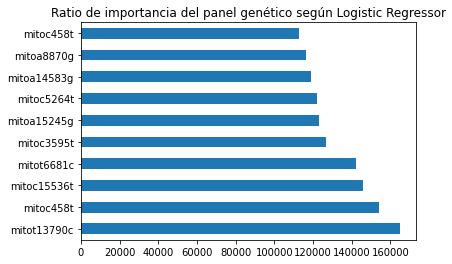
\includegraphics[width=0.45\textwidth]{importancia_rl_control1}
  \caption{Ratio de importancia Regreción Logística en el primer control}
  \label{fig:k-nn-example}
\end{figure}


\endinput
%------------------------------------------------------------------------------------
% FIN DEL CAPÍTULO. 
%------------------------------------------------------------------------------------
